\documentclass{article}

\usepackage[margin=1in]{geometry} 
\usepackage{amsmath,amsthm,amssymb,amsfonts, fancyhdr, color, comment, graphicx, environ,bbm}
\usepackage[dvipsnames]{xcolor}
\usepackage{subcaption}
\usepackage{mdframed}
\usepackage[shortlabels]{enumitem}
\usepackage{indentfirst}
\usepackage{hyperref}
\usepackage{placeins}
\usepackage{comment} %Comment large blocks
\usepackage{xfrac}
\usepackage{float} % To use "H" to force tables to be where wanted
\usepackage{booktabs} % Makes output from knittr:kable look better
\usepackage{parskip} %No indents for paragraphs
\usepackage[shortlabels]{enumitem} % To enumerate with letters
\hypersetup{
 colorlinks=true,
 linkcolor=blue,
 filecolor=magenta, 
 urlcolor=blue,
}
\pagestyle{fancy}
\usepackage{todonotes}

\newcommand{\E}{\mathbb{E}}
\renewcommand{\H}{\mathcal{H}}
\renewcommand{\L}{\mathcal{L}}
\newcommand{\dU}[1]{\ensuremath\frac{\partial u}{\partial #1}}
\newcommand{\dV}[1]{\ensuremath\frac{\partial v}{\partial #1}}
\newcommand{\ppx}[2]{\ensuremath\frac{\partial #1}{\partial #2}}
\newcommand{\ddx}[2]{\ensuremath\frac{d #1}{d #2}}
\newcommand{\indp}{\perp\!\!\!\perp} 

%\usepackage{mathpazo} %Dylan's fancy math bullshit that I don't want
\usepackage{microtype}
\usepackage{graphicx}
\usepackage{setspace}

%Footnote without a number
\newcommand\blfootnote[1]{%
  \renewcommand\thefootnote{}\footnote{#1}%
  \addtocounter{footnote}{-1}%
}

% Problem formatting [Alex]

\newenvironment{problem}[1]
    { \begin{mdframed}[backgroundcolor=Periwinkle!20] \textbf{(#1)} }
    {  \end{mdframed}}
% Define solution environment
\newenvironment{solution}{\textbf{Solution}\\}

%%%%%%%%%%%%%%%%%%%%%%%%%%%%%%%%%%%%%%%%%%%%%
%Fill in the appropriate information below
\lhead{Problem Set 1}
\rhead{Empirical Analysis} 
\title{Problem Set 1}
\author{Alex Weinberg \and Isaac Norwich \and Jose M. Quintero}

%%%%%%%%%%%%%%%%%%%%%%%%%%%%%%%%%%%%%%%%%%%%%
\begin{document}
\maketitle

Our code can be found in this GitHub respository: \url{https://github.com/jmquintero925/Metrics-III/tree/main/ps1Heckman}


%%%%%%%%%%%%%%%%%%%%%%%%%%%%%%%%%% QUESTION 1 %%%%%%%%%%%%%%%%%%%%%%%%%%%%%%%%%
\section*{Problem 1}
Comment on Richard Feynman’s commentary on social science and John Geweke’s further claim that most empirical papers in economics are wrong.
\begin{problem}{a}
What are the rewards to the author for doing careful empirical research?
\end{problem}
\begin{problem}{b}
Should empirical economic analysts be required to submit pre-analysis
plans before conducting research?
\end{problem}
\begin{problem}{c}
Explain how Bayesian, likelihood, and classical statistical inference approaches differ in learning from data.
\end{problem}
\begin{problem}{d}
 Read the papers by Christensen and Miguel (2018) and Chang and Li (2015). In light of results reported in these papers, is Feynman right? Is economics a pseudoscience?
\end{problem}


\newpage
%%%%%%%%%%%%%%%%%%%%%%%%%%%%%%%%%% QUESTION 3 %%%%%%%%%%%%%%%%%%%%%%%%%%%%%%%%%
\section*{Problem 2}
What is the “credibility approach” in economics? See, e.g., the Angrist
(2022) and Card (2022) Nobel lectures, as well as Hull et al. (2022)
\begin{problem}{a}
How is credibility defined? What are its ingredients?
\end{problem}

The credibility approach is defined as a having a transparent empirical strategy applied to concrete causal questions. The ingredients are isolating a source of variation in order to reveal causal effects of a specific policy on clearly defined outcomes. Focusing on sources of omitted variable bias and selection issues are important to this approach, while it does not focus on uncovering what some may call the ``true model'' that generates the data. 

\begin{problem}{b}
What mode of inference is implicitly invoked in the credibility papers?
\end{problem}

The mode of causal inference implicitly invoked in the credibility papers is one of controlled variation. That is, variation in treatment holding other factors constant is used to determine causal impacts of a policy. This is done in the framework of identifying causal models from actual data, where sampling variability is an issue. The goal is to recover a given model or desired counterfactual from a given set of data, not to model explicitly the choices made by individuals within the data. 

As Hull et al. (2022) state, the credibility approach is founded on the careful consideration of where the variation in the ``treatment'' in the research design originated in order to leverage this understanding to construct an appropriate comparison group. They state that this design-based approach can make transparent the key assumptions that drive the conclusion and guides the study's empirical validation or falsification.


Inherent in this approach is constructing counterfactuals that are based on appeals to intuition and not formal models. The mechanisms that determine how hypothetical counterfactuals are realized or how hypothetical interventions are implemented are not clearly specified. Instead, researchers using this mode of inference compare ``randomized'' to ``non-randomized'' (in quotes since in settings of quasi-experimental variation, the individuals are not explicitly randomized) interventions among individuals in their sample. These models depend on \textit{a priori} assumptions and cannot answer all of the relevant causal questions, as described in Heckman (ISR 2008, and in the lecture slides).


\begin{problem}{c}
What is the role of economic theory in doing “credible” empirical work? Should economists let theory get in the way of “letting the data speak”?
\end{problem}

In ``credible'' empirical work, the role of economic theory is in determining what factors impact the variation in the data. In fact, this is an interplay between letting the data speak and using economic theory. Researchers who use this approach use their understanding of economics and the institutional settings of the data in order to tease out the quasi-experimental variation they hope to leverage.

A short-coming to the ``credible'' approach is that these models are not capable of explaining why observationally identical individuals make different choices or even why they have different outcomes given the same choice. They do model that these observationally identical individuals have heterogeneous outcomes, but there is not underlying theory as to why this may be the case. In addition, the models don't draw a distinction between what the econometrician is able to see in the data versus the information set of the individuals being studied, even though this distinction is important in correcting for any selection. As discussed in class, another drawback is the lack of modeling the ex ante beliefs that the individuals have of their outcomes. All of these issues are due to a lack of structure imposed by economic theory inherent in this approach. 

In terms of letting theory get in the way of letting the data speak, I think that economists \textbf{should} let theory get in the way. We should not rely on the data only to determine what relationships underlie the data we see. We should formulate a theory and then use the model and the data to test the theory and estimate the parameters of said theory. If we then are able to reject said theory, we can test a different theory against the data. But we should not ignore theory when it comes to doing ``credible'' empirical work, since it is needed in order to design counterfactuals and to provide discipline on empirical work.

\newpage

%%%%%%%%%%%%%%%%%%%%%%%%%%%%%%%%%% QUESTION 3 %%%%%%%%%%%%%%%%%%%%%%%%%%%%%%%%%
\section*{Problem 3}
Consider a standard Cobb-Douglas production function:
\begin{align}\label{eq:eq1p3}
Y=A K^{\alpha} L^{\beta}, \quad \alpha+\beta<1, \alpha>0, \beta>0
\end{align}
where $A$ is a Hicks-neutral productivity shock and $K$ and $L$ are capital and labor, respectively. $Y$ is output. Function (1) is assumed to be policy invariant (i.e., the parameters $A, \alpha$, and $\beta$ are invariant to policy changes). Economists since Frisch call this property autonomy (see, e.g., Heckman, 2008, on the reading list and the April 28, 2022, lecture on causality). It is also structural in the sense of Hurwicz (1962). Define the outcomes $Y(k, l, a)$ as $Y$ when $K=k, L$ is fixed at $l$, and $A$ is fixed at $a . Y\left(k^{\prime}, l, a\right)$ is $Y$ when $K=k^{\prime}, L=l$, and $A=a$.
 
\begin{problem}{a}
Are $Y(k, l, a)$ and $Y\left(k^{\prime}, l, a\right)$ potential outcomes? Outputs of a structural model? What is the difference? What is the difference between a causal parameter and comparisons of structural functions evaluated at different points of their arguments? What is the causal effect of $k \rightarrow k^{\prime}$ ? What is ATE for a policy of fixing $K=k$ and $K=k^{\prime}$ ? How is it related to the marginal product of $k$ ?
\end{problem}

\begin{problem}{b}
Explain the difference between fixing $K$ and conditioning on it? When are they the same? When different? (Use a regression of (1) in logs to make your points.)
\end{problem}

\newpage
\section*{Problem 4}
Simulate a normal Generalized Roy model using the parameters used by Figure 1 in Heckman et al. (2006). Use samples of size 1000 .
\begin{problem}{a}
Compute ATE, TOT, MTE, for values of $\operatorname{Cov}\left(\frac{Y_{0}}{\sigma_{0}}, \frac{Y_{1}}{\sigma_{1}}\right)$ ranging from 1 to $-1$ in steps of $.10$.
\end{problem}
\begin{solution}
Begin by noting that
\begin{align*}
    \cov\left(\frac{Y_0}{\sigma_0},\frac{Y_1}{\sigma_1}\right) &= \cov\left(\frac{\alpha + U_0}{\sigma_0},\frac{\alpha+\beta + U_1}{\sigma_1}\right) \\ &=\cov\left(\frac{U_0}{\sigma_0},\frac{U_1}{\sigma_1}\right) \\
    &=\rho_{01}
\end{align*}
Thus during this exercise we will do comparative over the correlation of the two errors. Note that. since we are assuming a functional form we can calculate an analytic form for the MTE. Begin by noting 
\begin{equation*}
    U_1-U_0\sim\mathcal{N}(0,2(1-\rho_{01}))
\end{equation*}
Then, by definition the MTE is 
\begin{align*}
    MTE(u)= \E[Y_1-Y_0\vert U_D= u] &= \beta + \E[U_1-U_0\vert U_D = u] \\ 
    &= \beta + \E\left[U_1-U_0\Big\vert \Phi\left(\frac{U_0-U_1}{2(1-\rho_{01})}\right) = u\right] \\ 
    &= \beta + \E[U_1-U_0\vert U_1-U_0 = -2(1-\rho_{01})\Phi^{-1}(u)] \\ 
    &= \beta -2(1-\rho_{01})\Phi^{-1}(u)
\end{align*}
As a sanity check, we compare the results of the simulation with the analytic counterpart in Figure \ref{ps1H:q4:fig1a}. 
\begin{figure}[htb]
    \centering
    \caption{Marginal Treatment Effect}
    \label{ps1H:q4:fig1}
    \begin{subfigure}[b]{0.43\textwidth}
         \centering
         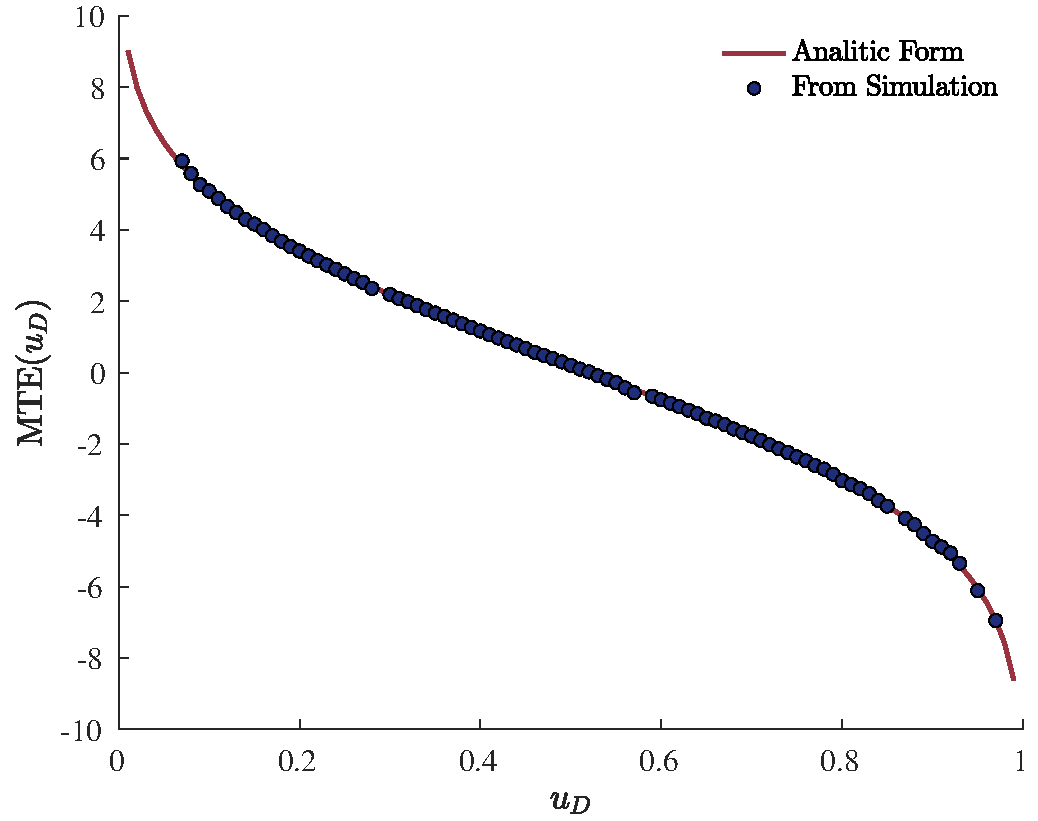
\includegraphics[width=\textwidth]{ps1Heckman/Figures/MTEcompare.pdf}
         \caption{Simulation vs. Analytic}
         \label{ps1H:q4:fig1a}
     \end{subfigure}
     \begin{subfigure}[b]{0.43\textwidth}
         \centering
         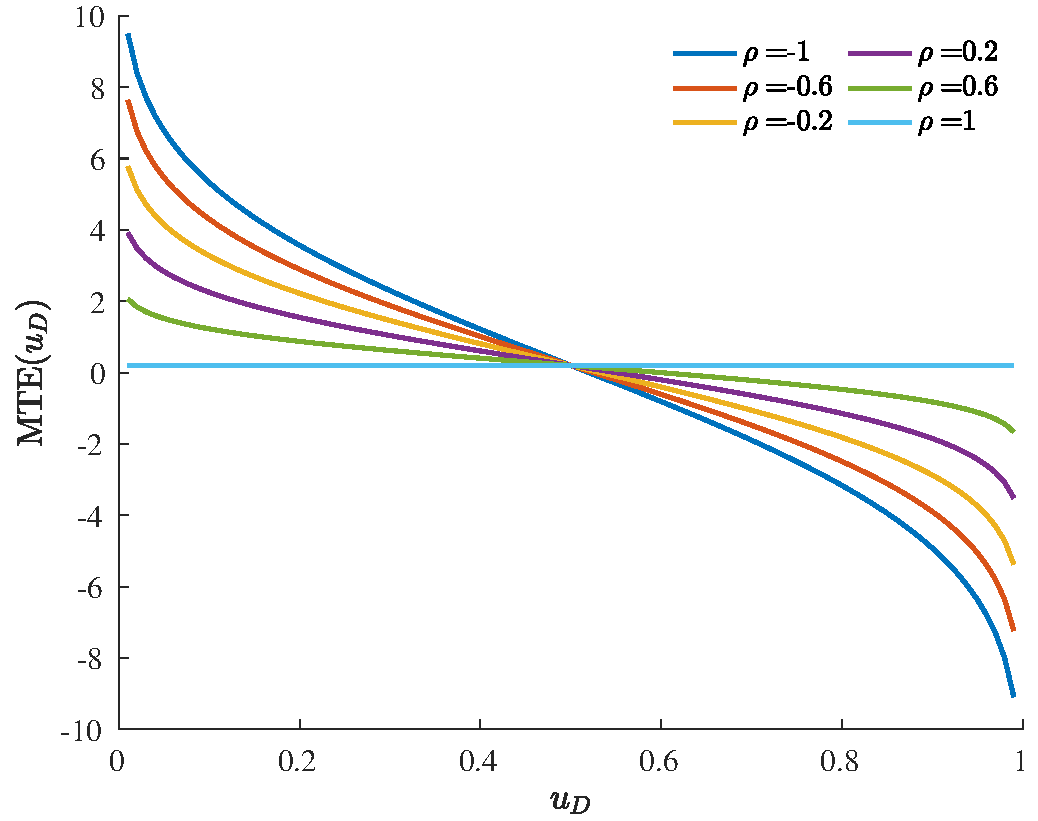
\includegraphics[width=\textwidth]{ps1Heckman/Figures/MTEgrid.pdf}
         \caption{Compare while varying $\rho$}
         \label{ps1H:q4:fig1b}
     \end{subfigure}
\end{figure}
\FloatBarrier
Next, we plot the MTE for different values of $\rho_{01}$. This results are presented in \ref{ea3:ps1:q3b:fig1}. Note as the correlation approaches to 1 the MTE approaches a flat curve around 0. When $\rho_{01}=1$ there is no gains in unobservables and thus no selection in unobservables. the rest of the treatment effects are presented in Figure \ref{ps1H:q4:fig2}. 
\end{solution}
\begin{problem}{b}
For each case, give LATE for a unit downward change in $C=.5$.
\end{problem}
\begin{solution}
\begin{figure}[htb]
    \centering
    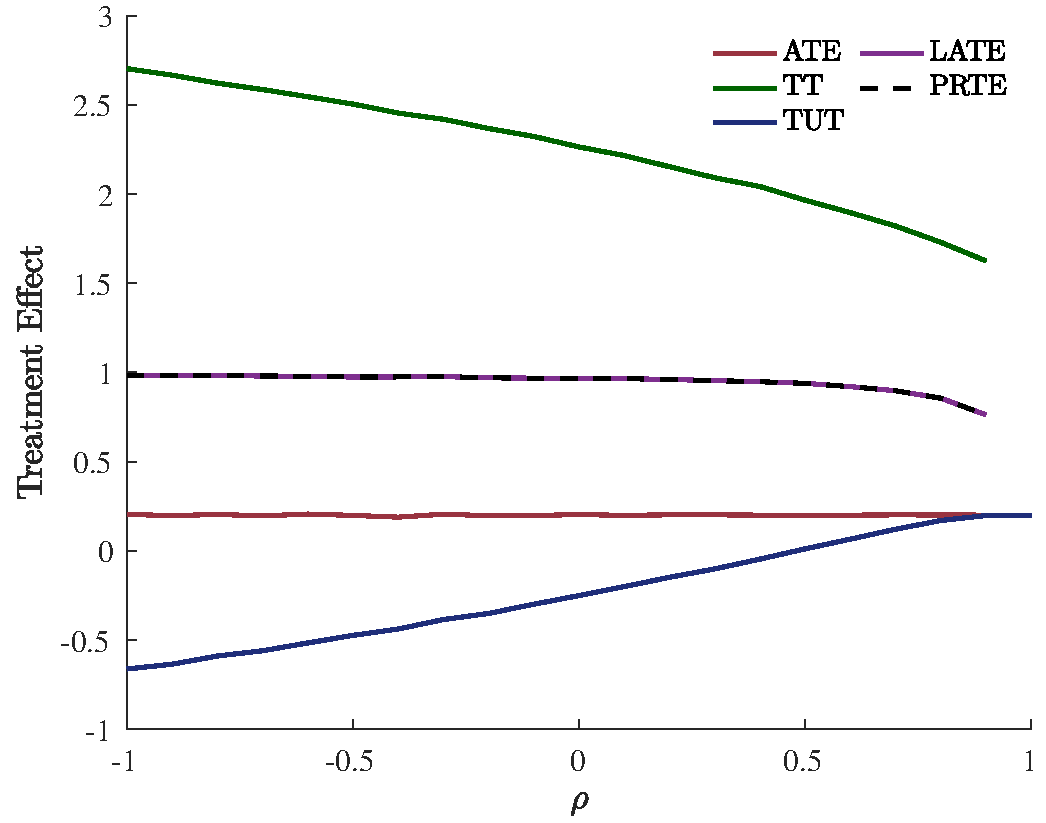
\includegraphics[width=0.45\textwidth]{ps1Heckman/Figures/treatments.pdf}
    \caption{Treatment effects}
    \label{ps1H:q4:fig2}
\end{figure}\end{solution}
\begin{problem}{c}
What is PRTE for a unit downward change in $C$ ?
\end{problem}
\begin{solution}
See Figure \ref{ps1H:q4:fig2}
\end{solution}
\begin{problem}{d}
Write this model as a random coefficient regression model with $Y=D Y_{1}+(1-D) Y_{0}$ as the dependent variable. $D=1$ corresponds to being in Sector $1 ; D=0$ otherwise. When is least squares a consistent estimator of ATE? TOT?
\end{problem}
\begin{solution}

\end{solution}


\newpage
\section*{Problem 5}
Isaac Newton demonstrated that gravity obeys the following relationship between two objects with masses $m_{1}$ and $m_{2}$ that are $r$ meters apart:
\begin{align*}
\text{Force:} \quad f=G \frac{m_{1} m_{2}}{r^{2}}
\end{align*}
where $G$ is a gravitional constant. Coulomb later found a similar relationship for electrical charge.
\begin{problem}{a}
Should we discard these laws because they are too functionally form-dependent?
\end{problem}
No, we shouldn't. We should test the implications of the functional form assumptions against data that we can collect. If the laws perform well given the observed data, then their testable hypotheses can be sustained. If there are circumstances under which the laws do not hold, then we can qualify their usefulness to just the scenarios where they are sustained. There's nothing specific about the functional form dependency by istelf that is objectionable.

\begin{problem}{b}
Equation \eqref{eq:eq1p3} in problem (3) is widely used in economics. For example, Hsieh and Klenow (2009) use it to study misallocation of inputs into manufacturing in India and China. It is a tool in trade in macro and IO. TFP is linked to this model. What is the evidence of Hsieh and Klenow on the validity of the Cobb-Douglas assumption? Does it matter? Should we reject studies based on a Cobb-Douglas function when a large body of evidence supports a CES technology instead?
\end{problem}
Hsieh and Klenow (2009) provide no evidence on the validity of the Cobb-Douglas assumption. They do, however, provide instances where this assumption forces specific results, such as on page 1425 where they state that "Cobb-Douglas aggregation across sectors means that TFPR equalization does not affect the allocation of inputs across sectors." If we would not want this to be an assumption baked in to the model, then perhaps we would use a different production function. They also discuss on pgs 1425-1426 the implications of using a CES aggregate of sector outputs as the final output and how it impacts their results.

Even though they do not provide evidence on the validity of the Cobb-Douglas assumption, we should not reject this or other studies. Instead, we should consider how dependent on the assumption the results are and consider the assumption by itself. If it really is true that a large body of evidence supports a CES technology instead, then I don't see why they would construct their model using Cobb-Douglas.

\begin{problem}{c}
Show how to test the Cobb-Douglas assumption with data like that of Hsieh and Klenow (2009). Is their evidence causal?
\end{problem}

To test Hsieh and Klenow (2009)'s assumption of a constant returns Cobb-Douglas production function, we can run an F-test that the exponents sum to 1. To do this, we would use their data and manipulate it to run a regression of $\ln Y$ on $ \sum_{s=1}^S \theta_s Y_s$. We would then test the null that $\sum_{s=1}^S \theta_s = 1$ using an F-test. If we reject the null, then we can say that the production function with constant returns to scale does not fit the data. 

However, this is a test of the \textit{type} of Cobb-Douglas production function, not of the choice of Cobb-Douglas over another type of production function. We can do a similar test for a different production function and compare the two head-to-head.

Their evidence can be thought of as causal if we think that that their assumptions are valid. Only under these assumptions do they identify causal results. Without evidence to the validity of the Cobb-Douglas assumption, we cannot say anything about the causal nature of their evidence, so in this case the answer is to be determined. Or rather, given that there is a ``large body of evidence support[ing] a CES technology instead [of a Cobb-Douglas technology]'' as stated in Part B, then we should absolutely not take their evidence to be causal.




\end{document}
